\chapter{The Short Baseline Neutrino Program}
\label{chap:SBN Program}
Results from LSND, MiniBooNE etc. at odds with null results from e.g. KARMEN and MINOS.. Need a definitive test.

Good stepping stone for DUNE - similar design (LArTPC)


\section{SBN Program Overview}

\begin{figure}
    \centering
    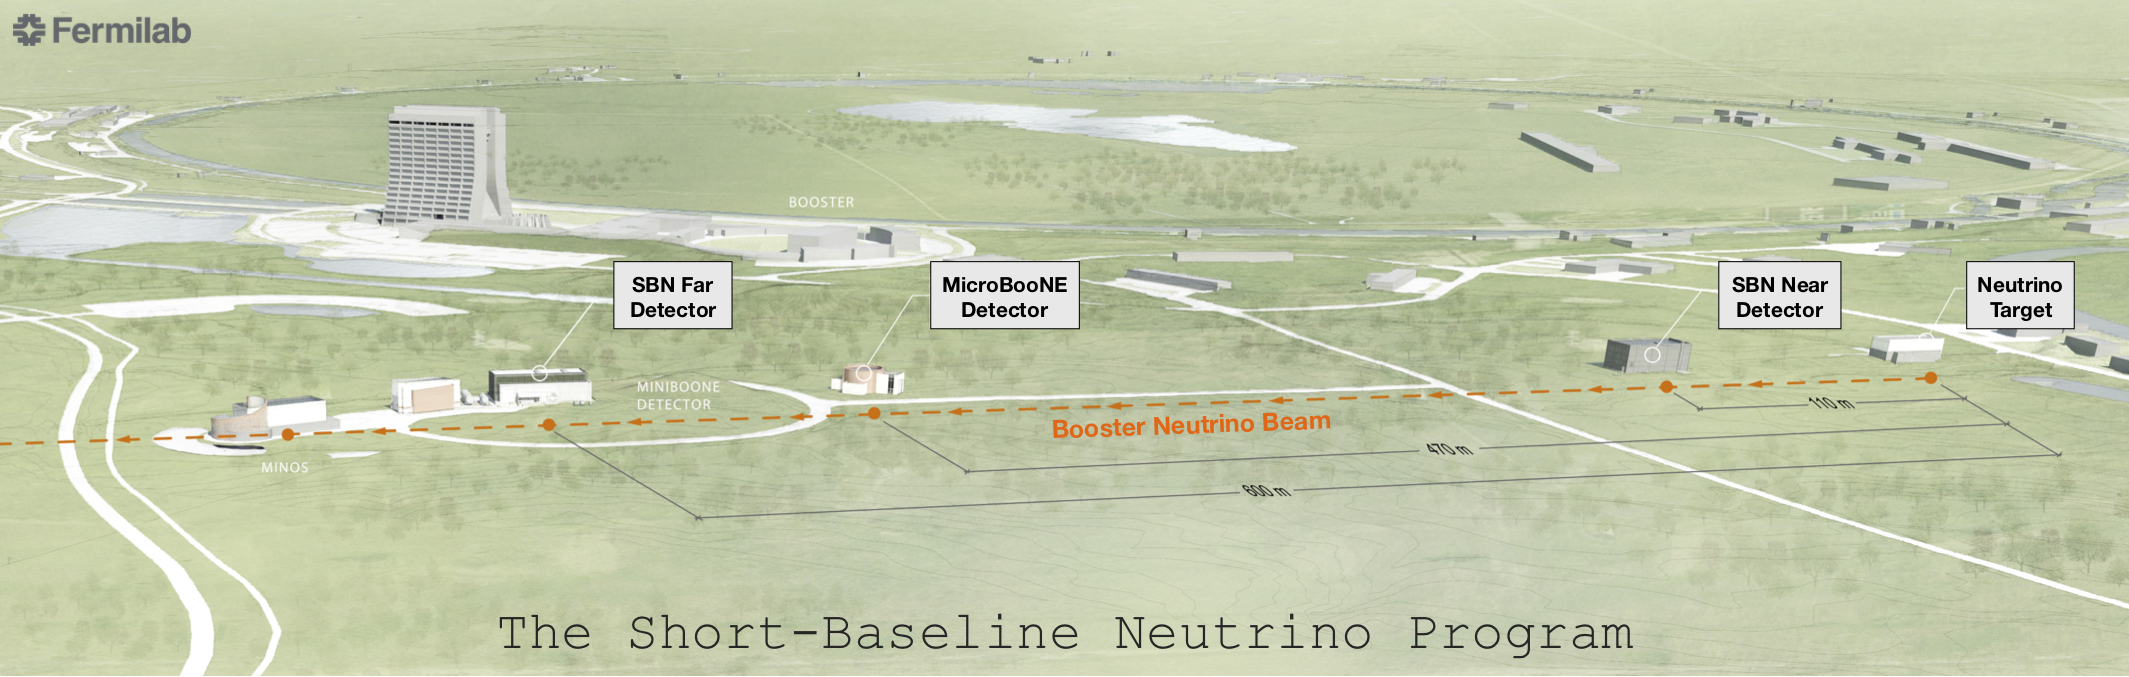
\includegraphics[width = \largefigwidth]{figures-chap3/SBN_program.jpg}
    \caption[SBN map.]{A view of the Fermilab complex highlighting the position of the \gls{sbn} detectors \cite{SBN_paper}.}
    \label{fig:my_label}
\end{figure}

The \gls{sbn} program is comprised of three distinct \gls{lartpc} type detectors located at the \gls{fnal}. The three detectors are \gls{sbnd}, \gls{microboone} and \gls{icarus} and all three lie along the axis of the \gls{bnb}. In order to minimise systematic uncertainties, the three detectors share many of the same technologies, the details of which are discussed in \SectionRef{sec:SBND} (\gls{sbnd}), \SectionRef{sec:MicroBooNE} (\gls{microboone}) and \SectionRef{sec:ICARUS} (\gls{icarus}). The \gls{bnb} consist predominantly of muon neutrinos with energies of the order 1 GeV and is discussed in detail in \SectionRef{sec:BNB}. The three detectors are positioned at 110m, 470m and 600m from the neutrino beam source respectively \cite{SBN_paper}. 

One of the primary aims of the \gls{sbn} program is to provide a definitive test to either confirm or refute the existence of light sterile neutrinos which have been hinted at by a number of experiments discussed in \SectionRef{subchap:Motivation for Sterile Neutrinos}. Other major aims of the \gls{sbn} program include investigating neutrino argon cross sections and developing large scale \gls{lartpc} technologies. The close proximity of \gls{sbnd} to the \gls{bnb} source means that \gls{sbnd} will observe neutrino argon interactions with high statistics allowing statistical uncertainties to be minimised and will allow for the exploration of rare channels such as neutrino-electron scattering. Both the development of \gls{lartpc} technology and an improved understanding of neutrino interaction cross-sections will be invaluable for future neutrino experiments such as the \gls{dune} \cite{SBN_paper}.


\section{Liquid Argon Time Projection Chambers}

The idea of a \gls{lartpc} was first proposed in 1977 by Rubbia in an attempt to consolidate the high resolution but low number of interactions obtained from 'bubble chamber' style detectors and the high rate but low resolution interactions obtained from 'counter' experiments. This would be achieved by propagating the complete image of an event through a noble element and then electronically reconstructing the 3D event by combining the 2D information collected and the drift time \cite{LArTPC_proposal}.

Liquid argon was identified as the most suitable medium to use for such a detector due to the following properties \cite{LArTPC_proposal}; 
\begin{itemize}
    \item High density (1.4 gcm$^{-3}$) with a sufficiently high atomic mass to allow for a reasonable probability of neutrino interactions.
    \item Argon is a noble element, meaning the electrons will not combine with the argon resulting in long drift times.
    \item A high electron mobility, meaning the electrons may drift quickly across the detector.
    \item Argon is relatively cheap and easy to purify.
    \item Argon may be liquefied easily using liquid nitrogen. 
\end{itemize}

\subsection{LArTPC Design}
The general design of a single chamber \gls{lartpc} is shown in \FigureRef{fig:lartpc}. Most \glspl{lartpc} consist of one or more \glspl{tpc} with a cathode and anode plane at either end inducing an electric field across the \gls{tpc}. The electric field causes charged particles to drift in the detector. The electrons produced from neutrino interactions will drift towards the anode where they will induce a current on a series of wire planes. The most rear wire plane (the one furthest away from the cathode) is known as the collection plane and the one or more wire planes in front of the collection plane are known as induction plane(s). There is a further potential difference between the induction and collection planes which ensures that the electrons will also reach the collection plane. The wire planes are orientated so that the wire angles between the planes are different which allows for 2D position reconstruction. Located behind the anode plane are also a series of \glspl{pmt} which collect scintillation light. The time taken for the scintillation light to be detected is very short in comparison to the time taken for the electrons to drift to the wire planes, so by using this timing information and knowing the electron drift velocity, the horizontal drift distance may be determined. Combining this with the 2D information from the wire planes allows for 3D event reconstruction. The induced current on the wire planes is interpreted in terms of signal waveforms from which \textit{hits} are constructed. Each hit contains information such as the associated wire plane, wire number and charge and it is this information which is used to obtain reconstructed information about an event \cite{Design_and_Construction_of_the_MicroBooNE_Detector}. The specific designs of the three \glspl{lartpc} used in the \gls{sbn} program are discussed in \SectionRef{sec:SBND} (SBND), \SectionRef{sec:MicroBooNE} (MicroBooNE) and \SectionRef{sec:ICARUS} (ICARUS).

\begin{figure}[h]
    \centering
    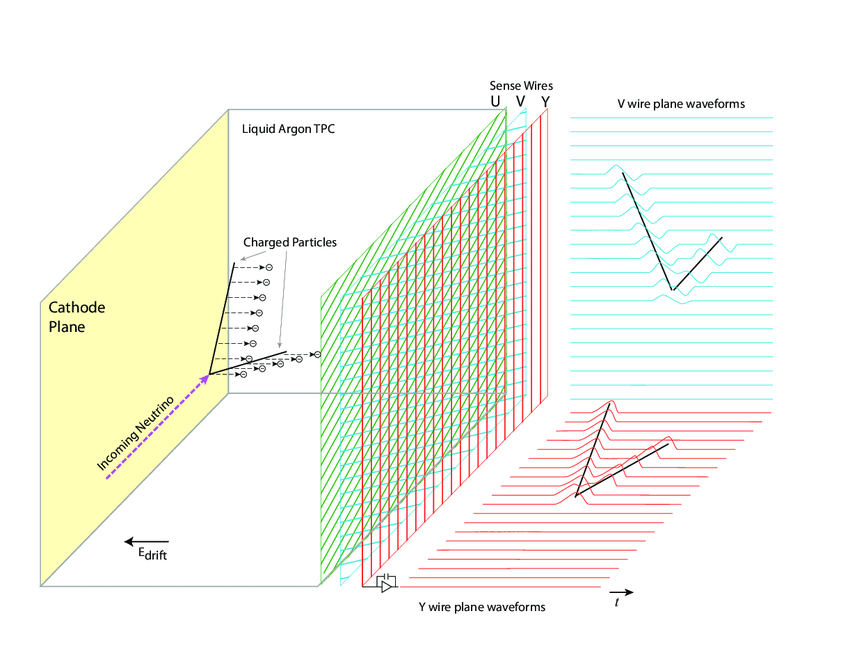
\includegraphics[width =\largefigwidth]{figures-chap3/Operational-principle-of-the-MicroBooNE-LArTPC.png}
    \caption[Schematic of LArTPC detector.]{A schematic of the operating principle of a \gls{lartpc} detector. A neutrino interacts in the argon producing secondary particles. The electric field across the \gls{tpc} causes charged particles to drift towards the wire planes where their energy deposits are recorded. \cite{Design_and_Construction_of_the_MicroBooNE_Detector}}
    \label{fig:lartpc}
\end{figure}
\newpage

\subsection{Detector effects}

Despite the many desirable properties of liquid argon, there are still a number of effects which have to be considered when performing event reconstruction.

\subsubsection{Diffusion}

Diffusion is the process in which the drifting electrons do not drift in such a way that they will continue to perfectly represent the initial image of an event. That is to say that the electrons will disperse as they drift in the detector. This happens in both the transverse and longitudinal directions with respect to the direction of the electric field and impacts the spatial resolution of the detector. 

For the case of a zero electric field and with the electrons in thermal equilibrium, the diffusion is isotropic and the diffusion coefficient, \textit{D}, is given by the Einstein relation such that
\begin{equation}
    D = \frac{kT}{e}\mu_0,
\end{equation}
where \textit{k} is Boltzmann's constant, \textit{T} is the temperature, \textit{e} is the elementary charge and $\mu_0$ is the electron mobility (for the case of no electric field).

In the presence of an electric field, the electron mobility is no longer given by $\mu_0$, but instead by $\mu$ and the electrons are no longer in thermal equilibrium. The diffusion also becomes anisotropic, leading to distinct diffusion coefficients for the longitudinal and transverse directions, $D_L$ and $D_T$ respectively which are given by
\begin{equation}
\begin{split}
    D_L &= \frac{kT}{e}(\mu + E \frac{\partial \mu}{\partial E}) \\
    D_T &= \frac{kT}{e}\mu.
\end{split}
\end{equation}
In general, the diffusion in the transverse direction is greater than the diffusion in the longitudinal direction \cite{LArTPC_book} \cite{diffusion}.

\subsubsection{Electron Lifetime}
 Electron lifetime is a measure of the free electrons lost due to attachment to impurities in the liquid argon whilst drifting across the detector \cite{ArgoNeuT_electron_lifetime_paper}. Naturally the electron lifetime, $\tau_{e}$, is coupled to the purity of the argon and is defined as 
 \begin{equation}
     \tau_{e} = 1/k_e,
 \end{equation}
 where $k_e$ is the impurity concentration. The rate of charge loss is then given by 
 \begin{equation}
     Q = Q_{0}e^{-t/\tau_e},
 \end{equation}
where $Q$ is the charge remaining after correcting for electron lifetime, $Q_0$ is the initial charge and $t$ is the drift time. 
 
\subsubsection{Recombination}
When argon atoms are ionised, the resulting ionised electron may immediately recombine with a nearby argon ion instead of being separated by the electric field in the detector. This is known as the recombination effect and the magnitude of the effect is largely determined by the local electric field. A number of different approaches to model the recombination effect exist, however for liquid argon detectors a form of the box model or Jaff\'{e} model are usually used \cite{LArTPC_book}.

The Jaff\'{e} model is based on the idea that recombination depends on the charge density of both nearby electrons and ions. The model assumes a cylinder surrounding the ionisation track and recombination may occur between any of the ionised electrons and ions, not just the electron with it's associated parent ion which is were the Jaff\'{e} model largely differs from earlier models \cite{Jaffe_model}. The recombination effect from the Jaff\'{e} model is given by 
\begin{equation}\label{Jaffe}
    Q = \frac{Q_{0}}{1+q_{0}F(Esin\phi)},
\end{equation}
where $Q_0$ is the initial charge, $Q$ is the charge after recombination, $q_0$ is the initial density of electron-ion pairs and $F$ is a function depending on the electric field $E$, the angle between the field and the ionisation track, $\phi$ and other quantities which describe the diffusion. \EquationRef{Jaffe} is commonly approximated by Birks' law with a normalisation parameter to help fit the model to the experimental data \cite{LArTPC_book}. 

In their development of the box model, Thomas and Imel assumed the diffusion and ion mobility to be zero and instead of the cylindrical column used in the Jaff\'{e} model, they considered a box with a uniform charge distribution such that, 
\begin{equation}
    Q = Q_{0}\frac{1}{\xi}ln(1+\xi),
\end{equation}
where $\xi = \alpha Q_0/E$. $\alpha$ is a free parameter and $Q$ and $Q_0$ are defined as in \EquationRef{Jaffe}\cite{LArTPC_book}\cite{Recombination_box_model}.


\subsubsection{Space Charge}
The electric field in a \gls{tpc} is usually designed to be uniform between the cathode and the anode, however, particularly for surface level detectors this often doesn't end up being the case. Cosmic muons may enter the detector ionising the argon atoms. The ionised electrons and argon ions then drift towards the anode and cathode respectively, however the drift time for the ions is much greater than the electron drift time. If the flux of cosmic muons entering the detector is sufficiently large, this results in a significant positive charge build up towards the cathode. This effect is known as \textit{space charge} and directly impacts the recombination effect since it is linked to the magnitude of local electric field as well as affecting the drifting electrons.

\textcolor{red}{SOME SPACE CHARGE MATH?}

\section{Booster Neutrino Beam}\label{sec:BNB}
The \gls{bnb} is produced by firing 8 GeV protons onto a beryllium target resulting in a secondary beam of hadrons. A toroidal focusing horn surrounds the target and focuses or defocuses charged particles depending on the sign of their charge. The focused hadrons then travel down a 50 m tunnel where most of them will decay producing muon neutrinos and small fraction of electron neutrinos. At the end of the 50 m decay region is a concrete and steel absorber designed to absorb any non-neutrino particles. A schematic of the \gls{bnb} layout is shown in \FigureRef{fig: BNB schematic}. The decay modes of the hadrons resulting in a neutrino and the corresponding branching ratios are listed in \TableRef{Table: BNB decay modes}. 

\begin{figure}
    \centering
    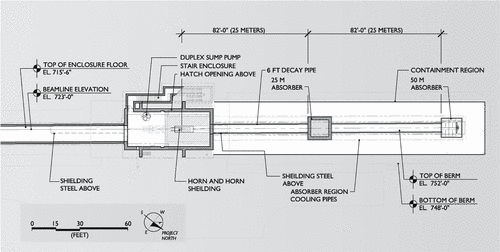
\includegraphics[width =\largefigwidth]{figures-chap3/BNB_schematic.png}
    \caption[Schematic of the BNB layout.]{A schematic of the layout of the \gls{bnb} \cite{BNB_flux}.}
    \label{fig: BNB schematic}
\end{figure}

\begin{table}[h]
\begin{tabular}{ccc}
Particle                 & Decay Mode                        & Branching Ratio (\%) \\ \hline
\multirow{2}{*}{$\pi^+$} & $\mu^+ + \nu_{\mu}$               & 99.9877             \\
                         & $e^+ + \nu_e$                     & 0.0123              \\ \hline
\multirow{3}{*}{$k^+$}   & $\mu^+ + \nu_{\mu}$               & 63.44               \\
                         & $\pi^0 + e^+ + \nu_e$             & 4.98                \\
                         & $\pi^0 + \mu^+ \nu_{\mu}$         & 3.32                \\ \hline
\multirow{4}{*}{$k^0$}   & $\pi^- + e^+ + \nu_e$             & 20.333              \\
                         & $\pi^+ + e^- + \bar{\nu}_e$         & 20.197              \\
                         & $\pi^- + \mu^+ + \nu_{\mu}$       & 13.551              \\
                         & $\pi^+ + \mu^- + \bar{\nu}_{\mu}$ & 13.469              \\ \hline
$\mu^+$                   & $e^+ + \nu_e + \bar{\nu}_e$       & 100                
\end{tabular}
\caption[Hadron decay mode in the BNB.]{The decay modes of the hadrons produced by the \gls{bnb} when running in neutrino mode. The branching ratio of each of the decay modes is also given \cite{BNB_flux}.}
\label{Table: BNB decay modes}
\end{table}

\newpage
A current of 174 kA is supplied to the magnetic horn in 143 $\mu$s pulses which corresponds to the frequency of the incident protons. The direction of the current may be reversed allowing for the focusing of positively or negatively charged particles. Since the charge of the decaying hadrons is linked to the type of neutrino produced, the ability to focus both positively and negatively charged particles allows the \gls{bnb} to run in neutrino or anti-neutrino mode. Pions are the primary particle produced from the incident protons hence the \gls{bnb} is muon (anti-)neutrino dominated. The percentage neutrino flavour composition of the \gls{bnb} is given in \TableRef{Table: BNB composition} for both neutrino and anti-neutrino mode.


\begin{table}[h]
\begin{tabular}{ccc}
Neutrino Flavour & \% in Neutrino Mode & \% in Anti-neutrino Mode \\ \hline
$\nu_\mu$        & 93.6                & 15.71                    \\
$\bar{\nu}_{\mu}$  & 5.86                & 83.73                    \\
$\nu_e$          & 0.52                & 0.2                      \\
$\bar{\nu}_{e}$    & 0.05                & 0.4                     
\end{tabular}
\caption[BNB flavour composition.]{The neutrino flavour composition of the \gls{bnb} when it's running in either neutrino or anti-neutrino mode \cite{BNB_flux}.}
\label{Table: BNB composition}
\end{table}

 The neutrino flux of the BNB was simulated by the MiniBooNE collaboration for both neutrino and anti-neutrino mode \cite{BNB_flux}. The flux of the electron and muon (anti-)neutrinos in each of the three \gls{sbn} detectors is shown in \FigureRef{fig: SBN flux}.
 \begin{figure}[h!]
     \centering
     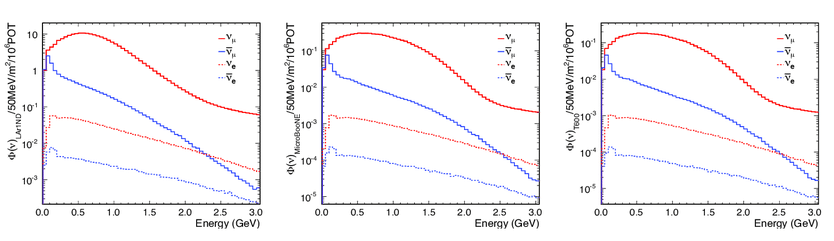
\includegraphics[width = \largefigwidth]{figures-chap3/SBN_flux.png}
     \caption[Neutrino fluxes in SBN.]{The predicted flux of the \gls{bnb} at \gls{sbnd} (left), \gls{microboone} (middle) and \gls{icarus} (right) for both electron and muon neutrinos and anti-neutrinos \cite{SBN_Proposal}.}
     \label{fig: SBN flux}
\end{figure}
The systematic uncertainties associated with the \gls{bnb} account for an error of $\sim 9\%$ at the peak of the $\nu_\mu$ flux with a larger error for energies either side of the peak. The systematic uncertainties are mainly due to determining the rate and spectrum of neutrinos for each proton on target, determining the rate and spectrum of secondary particles produced from protons interacting with the beryllium target, the rate of hadronic interactions, the focusing properties of the magnetic horn and the beamline geometry \cite{BNB_flux}. 



\section{SBND}\label{sec:SBND}
\gls{sbnd} was purposely designed to be the near detector of the \gls{sbn} program and has an active volume with dimensions (4, 4, 5) m containing 112 tons of liquid argon. It consists of two \glspl{tpc}, where the central shared cathode sits in the middle of the detector with an anode either side as is shown in \FigureRef{fig:sbnd_schematic}. Each of the \glspl{apa} consist of three wire planes where the first and second induction plane are orientated at $\pm 60^{\circ}$ to the vertical and the collection plane is vertical. In all cases, the wire plane spacing and the wire pitch are 3 mm. The nominal electric field in each of the \glspl{tpc} is 500 V/m. 

\begin{figure}[!h]
    \centering
    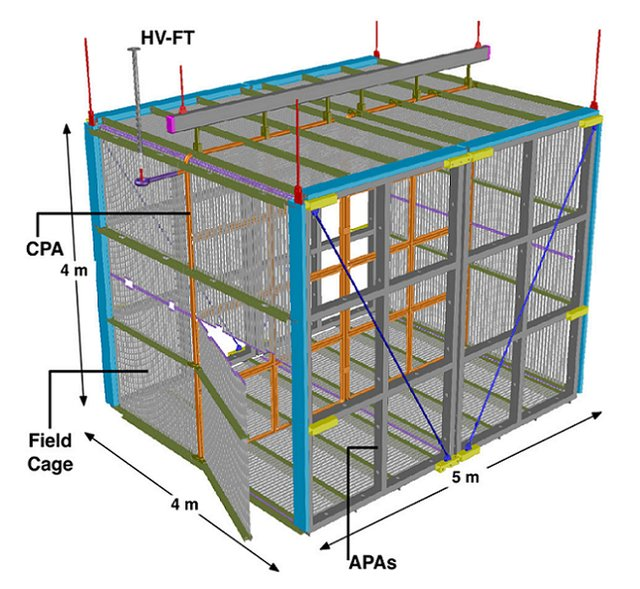
\includegraphics[width = \largefigwidth]{figures-chap3/SBND.jpg}
    \caption[Schematic of the SBN detector.]{Schematic showing the dimensions of the SBND detector. The \gls{cpa}, \glspl{apa} (only one is labelled) and field cage are shown. The \gls{pds} is not shown, but 12 squares on the near \gls{apa} represent the location where the \gls{pds} boxes will be positioned. \cite{LArTPC_review}}
    \label{fig:sbnd_schematic}
\end{figure}

\gls{sbnd} is considered to be a surface level detector with no overburden. Consequently, the cosmic ray flux will be significant with an average of 3 cosmic rays seen in each neutrino event \cite{SBN_Proposal}. This will be the most abundant background in \gls{sbnd} and therefore it will be crucial to be able to identify the cosmic ray muons. In order to do this, \gls{sbnd} will use a \gls{crt} system which consists of a total of 7 panels, one for each side of the detector plus an additional one for the top face as this is where most of the cosmic rays will be entering the detector from. \FigureRef{fig:sbnd_crt} shows how the \gls{crt} panels will be positioned. Each \gls{crt} plane consists of two layers, where one layer is comprised of 2$\times$5 X-oriented modules and the other layer is comprised of 2$\times$4 Y-oriented modules. Each of these modules is comprised of 16 scintillator strips which are in turn attached to \glspl{sipm}. The orthogonal two layer setup coupled with the \gls{sipm} readout allows the the location of an interaction in the \gls{crt} to be determined \cite{sbnd_crt}. The \gls{crt} system monitors the crossing time and coordinates of the particles and compares them with the information from the light detection system and the beam time rejecting the events identifies as cosmic muons. \cite{microboone_crt}.

\begin{figure}[!h]
    \centering
    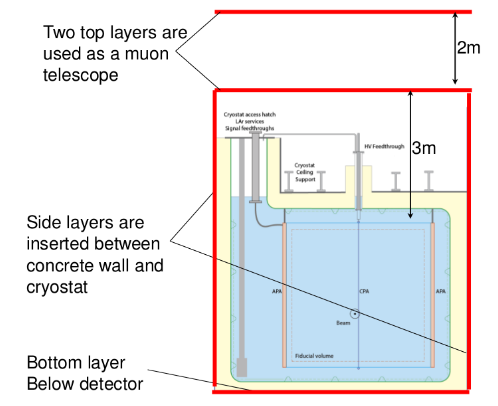
\includegraphics[width = \largefigwidth]{figures-chap3/SBND_CRT.png}
    \caption[CRT positioning in SBND.]{Diagram showing how the \gls{crt} will surround \gls{sbnd} on all sides with an additional panel above the top surface \cite{SBN_Proposal}.}
    \label{fig:sbnd_crt}
\end{figure}

\textcolor{red}{READOUT ELECTRONICS?? KNOW LITERALLY NOTHING ABOUT THIS..}

%\subsection{Photon Detection System}
The \gls{pds} consists of a total of 24 \textit{boxes}, 12 of which will be mounted behind each \gls{apa}. Each box houses 5 \glspl{pmt} and 8 \glspl{arapuca} (specifically, X-ARAPUCA's are used which are an advancement over the initial \gls{arapuca} design) as shown in \FigureRef{fig:pds_box}. The 4 outer \glspl{pmt} of each box are coated with \gls{tpb} whilst the central one remains uncoated. The scintillation light produced has wavelengths in the \gls{vuv} region, however the \glspl{pmt} are only able to detect visible light. The \gls{tpb} coating shifts the wavelength of the \gls{vuv} light into the visible region allowing it to be detected. Therefore, the coated \glspl{pmt} are sensitive to both visible and \gls{vuv} light whilst the uncoated \glspl{pmt} are only sensitive to visible light \cite{LArTPC_review}. 

\glspl{arapuca} are a novel light trap which consist of a box where the internal surfaces are highly reflective. The surface of the \gls{arapuca} which faces the incoming light consists of dichroic filter with a wavelength shifter either side of the filter. The wavelength of the light which is incident on the outermost shifter is shifted such that it may pass through the dichroic filter and after passing through the filter the light is again wavelength shifted so that it may no longer pass through the filter and thus remains trapped in the \gls{arapuca}. A schematic of the \gls{arapuca} design is shown on the left of \FigureRef{fig:arapuca}. The inside of the \gls{arapuca} module contains a \gls{sipm} photo-sensor in order to detect the light. Due to the highly reflective nature of the inside of the \gls{arapuca}, only a small region needs to be exposed to a photo-sensor in order to detect the trapped photons \cite{ARAPUCA}. The X-ARAPUCA improves on the initial design by replacing the inner wavelength shifter with an acrylic slab with the wavelength shifter implanted in the slab and the photo-sensor being directly attached to the slab. Light entering the X-ARAPUCA may be detected in same way as was done in the original \gls{arapuca} (\FigureRef{fig:arapuca}: Left), however the photons may also become trapped in the slab by total internal reflection and travel within the slab to the photo-sensor (\FigureRef{fig:arapuca}: Middle) or if the light enters at a large angle, the photons may become trapped between the surface of the slab and the filter and will travel to the photo-sensor without ever entering the slab (\FigureRef{fig:arapuca}: Right). The middle scenario of \FigureRef{fig:arapuca} represents a direct improvement over the original \gls{arapuca} design because the number of reflections on the internal sides of the X-ARAPUCA module is reduced which in turn increases the photon detection efficiency \cite{X-ARAPUCA}. 

\begin{figure}[!h]
    \centering
    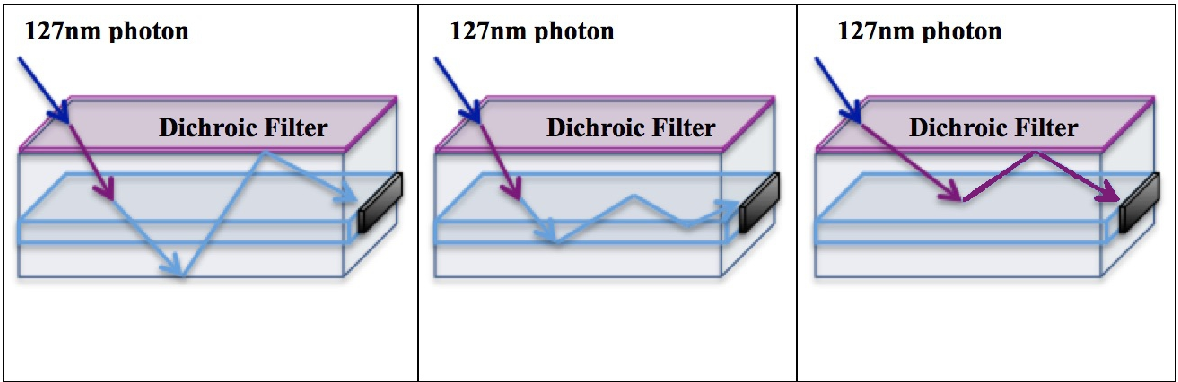
\includegraphics[width = \largefigwidth]{figures-chap3/arapuca.png}
    \caption[ARAPUCA operating principle.]{The three possibilities for trapping light in an X-ARAPUCA. Left: The standard \gls{arapuca} design. Light is wavelength shifted in order to pass through the dichroic filter. Once passed the filter, it is wavelength shifted again so that may not exit through the filter again. The photons are reflected within the \gls{arapuca} until they are detected by the photo-sensor. Middle: an acrylic slab containing the inner wavelength shifter is placed in the X-ARAPUCA and the photo-sensor is attached to the slab. Light may be become trapped within the slab by total internal reflection. Right: Incident light at a large angle may become trapped between the surface of the slab and the filter \cite{X-ARAPUCA}.}
    \label{fig:arapuca}
\end{figure}

Another component of the \gls{pds} is covering each side of the \gls{cpa} with a 19 m$^2$ of \gls{tpb} coated reflective covering. This means that \gls{vuv} light directed towards the \gls{cpa} will be wavelength shifted into the visible spectrum and reflected back to towards the \glspl{pmt} where it may be detected. Since one of the \glspl{pmt} in each of the boxes remains uncoated, it will allow \gls{sbnd} to distinguish between light that is initially directed towards the \glspl{pmt} and the reflected light because the reflected light will be visible in all \glspl{pmt} whereas only the four outer \glspl{pmt} will be able to detect direct light \cite{LArTPC_review}. 

\begin{figure}[!h]
    \centering
    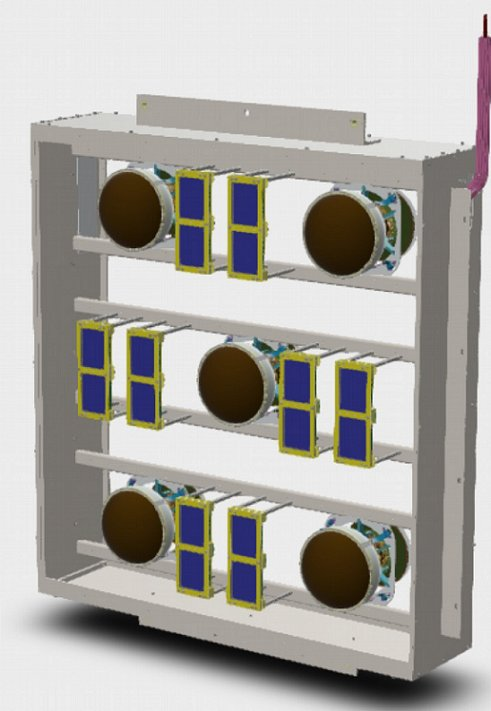
\includegraphics[width = \largefigwidth]{figures-chap3/PDS_box.jpg}
    \caption[Schematic of PDS box.]{Schematic of the \gls{pds} box showing the position of the 5 \glspl{pmt} and the 4 pairs of X-ARAPUCA'S. The central \gls{pmt} is left uncoated, whilst the 4 outer \glspl{pmt} are coated with \gls{tpb} \cite{LArTPC_review}.}
    \label{fig:pds_box}
\end{figure}

\section{MicroBooNE}\label{sec:MicroBooNE}

The \gls{microboone} detector is located slightly upstream of its predecessor, \gls{miniboone}. The detectors are at 470 m and 500 m from the \gls{bnb} source respectively. The Principal design goal of \gls{microboone} is to investigate the low energy excess of events observed by \gls{miniboone} and it began its operations in 2015 were it was initially used as a stand alone detector before becoming part of the larger \gls{sbn} program \cite{microboone_detector}.

\begin{figure}[h!]
    \centering
    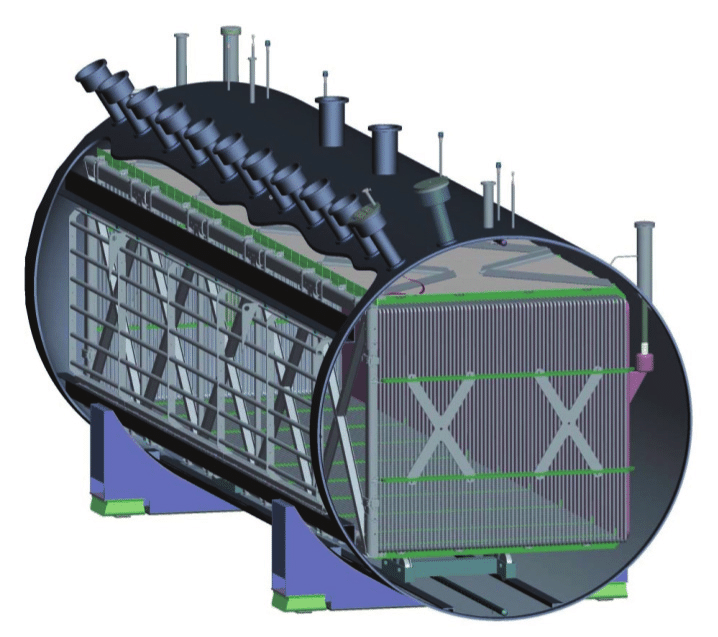
\includegraphics[width = \smallfigwidth]{figures-chap3/MicroBooNE.png}
    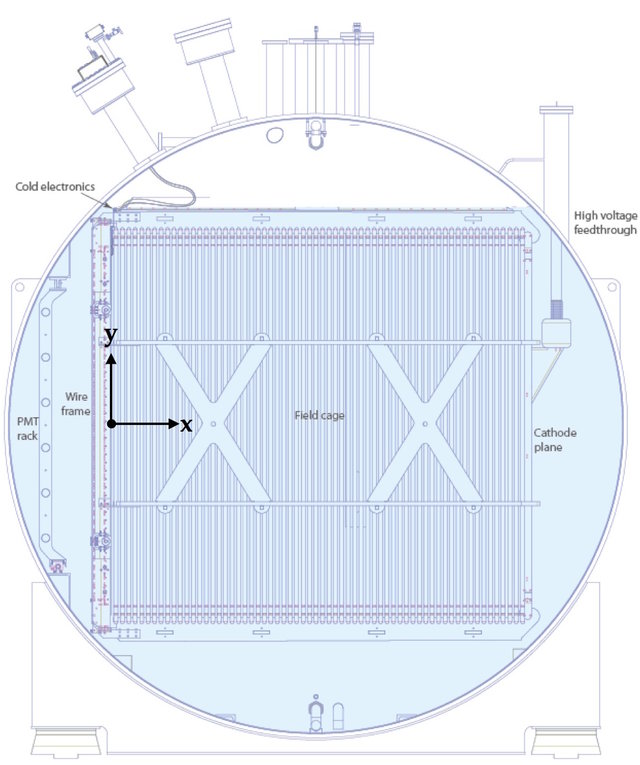
\includegraphics[width = \smallfigwidth]{figures-chap3/MicroBooNE_cross-section.jpg}
    \caption[MicroBooNE detector.]{Diagram of the \gls{microboone} \gls{lartpc} inside the cryostat with the open front and left side showing the field cage and anode planes respectively (Left). Cross-section schematic of the \gls{microboone} detector orientated such that the beam direction (z-direction) is orientated out of the page \cite{microboone_detector}.}
    \label{fig:microboone}
\end{figure}

The \gls{microboone} detector consists of a single \gls{tpc} enclosed within a cryostat as is shown in \FigureRef{fig:microboone}. The \gls{tpc} has dimensions of (2.560, 2.325, 10.368)~m and is orientated such that the z direction is along the neutrino beam line with the cathode to the left of the beam and the anode to the right. The active volume is defined as the volume enclosed by the \gls{lartpc} field cage which has a liquid argon mass of 90 tonnes out of a total 170 tonnes. The \gls{apa} consists of three wire planes with the wires on the two induction planes orientated at $\pm 60^{\circ}$ to the vertical and the wires of the collection plane orientated vertically. Both the wire plane spacing and the wire pitch of each plane is 3 mm. Unlike \gls{sbnd} and \gls{icarus}, the nominal electric field in \gls{microboone} is 273 V/cm. The light collection system consists of a series of 32 \glspl{pmt} and 4 lightguide paddles which are located directly behind the anode planes. The lightguides have a large collection area and their purpose is to guide light to the \glspl{pmt} (the lightguide paddles were disfavoured once the ARAPUCA technology was developed.)\cite{microboone_detector}.

\gls{microboone} is also considered a surface level detector being only $\sim 6$ m underground and as there is no overburden present, a large flux of cosmic rays are observed. A \gls{crt} system similar to the one described in \SectionRef{sec:SBND} for \gls{sbnd} was implemented. The \gls{crt} system consists of 73 scintillating modules, however it is only sensitive to the four sides of the X and Y coordinates of the detector. 








\section{ICARUS}\label{sec:ICARUS}

The \gls{icarus} detector was first operated in 2010 and  located at the Gran Sasso National Laboratory in Italy where it was used to detect events from cosmic rays and from the neutrino beam which is directed from CERN to Gran Sasso. In 2013 the decommissioning process began and the detector was taken to CERN for refurbishment before making its way to \gls{fnal} and becoming part of the \gls{sbn} program \cite{SBN_Proposal}.

The \gls{icarus} detector consists of two \textit{modules} within a single cryostat with each module containing two \glspl{tpc}. A schematic of this design is shown in \FigureRef{fig:icarus}. Similar to \gls{sbnd}, the two \glspl{tpc} within each module share a common cathode. The dimensions of each module are (3.6, 3.9, 19.6) m and the cryostat contains 760 tonnes of liquid argon with an active volume of 476 tonnes.  Again, the \glspl{apa} consists of three wire planes with a wire plane spacing and wire pitch of 3 mm. In contrast to \gls{sbnd} and \gls{microboone} however, the wire planes are orientated at 0$^\circ$ for the first induction plane and at $\pm 60^\circ$ for the second induction plane and the collection plane. The choice of having a horizontal wire plane is due to \gls{icarus} being initially designed to detect cosmic rays which would predominantly enter the detector from above and therefore be travelling perpendicular to the horizontal. The nominal electric field in each of the \glspl{tpc} is 500 V/m \cite{SBN_Proposal}. 

The light collection system for \gls{icarus} is comprised of a series of 74 \glspl{pmt} positioned behind the wire planes. The layout of the \glspl{pmt} is however asymmetric with the east module having a $3 \times 9$ array of \glspl{pmt} for each \gls{tpc} whereas the two \glspl{tpc} in the west module have a single row of 9 \glspl{pmt} plus two additional \glspl{pmt} located centrally above and below the main row in the right chamber. Since the light is again produced with wavelengths in the \gls{vuv} region, the \glspl{pmt} are coated with \gls{tpb} in order to shift the wavelength into the visible region \cite{SBN_Proposal}.  

\begin{figure}[h!]
    \centering
    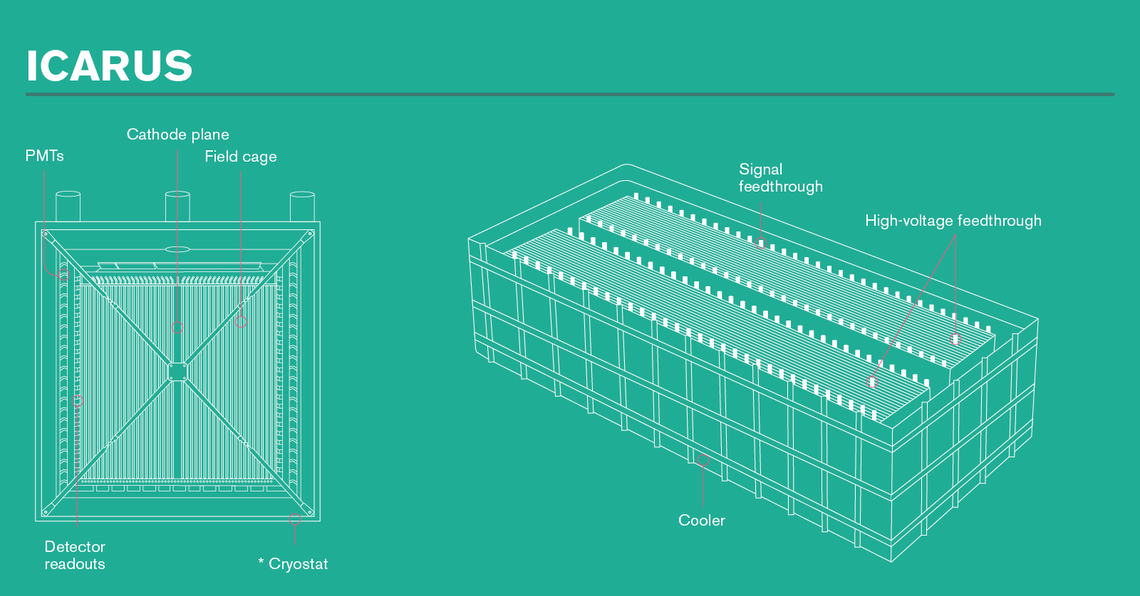
\includegraphics[width = \largefigwidth]{figures-chap3/icarus.png}
    \caption[ICARUS detector.]{Schematic of of the \gls{icarus} detector. The left image shows a cross-section of one of the two modules whereas the right images shows the whole detector with the the two modules side by side \cite{ICARUS_image}.}
    \label{fig:icarus}
\end{figure}

The \gls{icarus} \gls{crt} system surrounds the detector on all sides however the actual position is not always the same due to design choices. The \gls{crt} on the top most side which experiences the highest flux of cosmic rays, is located outside the \gls{tpc}, about 3m from the top face above the readout electronics. It consists of two planes of scintillating modules with the readout coming from the same electronics board as is used by \gls{sbnd}.
The \gls{crt} for the vertical sides are again outside the \gls{tpc} and behind the \gls{pmt} arrays and close to the cryostat walls. The scintillator modules from the \gls{minos} experiment are being reused for this purpose. The \gls{crt} for the bottom face are the repurposed spare modules from the veto shield from the Double Chooz experiment and are located within the cryostat. Only about 50\% of the bottom face is be covered by the \gls{crt} because of limited space due to the supporting structure of the cryostat \cite{SBN_Proposal}\cite{ICARUS_CRT}.

\section{SBN Physics Capabilities}

The \gls{sbn} program was designed with the aim of resolving the contentious results observed by a number of experiments as was discussed in \SectionRef{subchap:Motivation for Sterile Neutrinos}. Since it was purposely planned with this in mind, the \gls{sbn} program has a number of advantages over previous experiments in the hopes of detecting eV scale sterile neutrinos: it has a multi detector design, the near and far detector are positioned such that the oscillation signal is close to maximal for an expected set of oscillation parameters, the detectors use the same technology and have the same target medium. 

The top two plots of \FigureRef{fig:osc_probability} show the expected oscillation probability for the \nue appearance channel as a function of the baseline for two sets of oscillation parameters, $(sin^22\theta_{\mu e}, ~\Delta m^2_{41}) = (0.015, ~0.3~\text{eV}^2), (0.002, ~1.5~\text{eV}^2)$ and a neutrino energy of 700 MeV. The neutrino energy corresponds to the peak energy of the \gls{bnb} and the oscillation points are chosen as the upper and lower limits of the global \nue appearance data. In both cases there is a clear difference in the oscillation probability between the near and far detector showing that the \gls{sbn} program is sensitive to oscillations within this parameter range \cite{SBN_paper}. The bottom two plots show the oscillation probability for the same two oscillation points as a function of neutrino energy for baselines of 110 m and 600 m. The ratio of the oscillation probability at 600 m to that at 110 m is also shown. Again there is a clear difference in the oscillation probability for most energies showing that the \gls{sbn} program is sensitive to a wide range of neutrino energies \cite{SBN_paper}. The \nue appearance oscillation sensitivity constructed at the time of the proposal is shown in \FigureRef{fig:SBN_proposal_sensitivity}. These contours include the relevant backgrounds and systematic uncertainties with the exception of detector systematics. 

The event rates in the near and far detector are correlated since both use the same interaction medium and the same technology to detect interactions. As \FigureRef{fig:osc_probability} shows, \gls{sbnd} will observe no or very few oscillated events and will give a measure of the absolute flux and interaction cross-section whereas both \gls{microboone} and \gls{icarus} are able to detect oscillated events with significant probability. Typically the \gls{bnb} flux uncertainties and interaction cross-section uncertainties are fairly large, however, comparing results from \gls{sbnd} to \gls{microboone} and \gls{icarus} and noting the correlation between the detectors allows the uncertainties to be constrained \cite{SBN_paper}. 

\begin{figure}[!h]
    \centering
    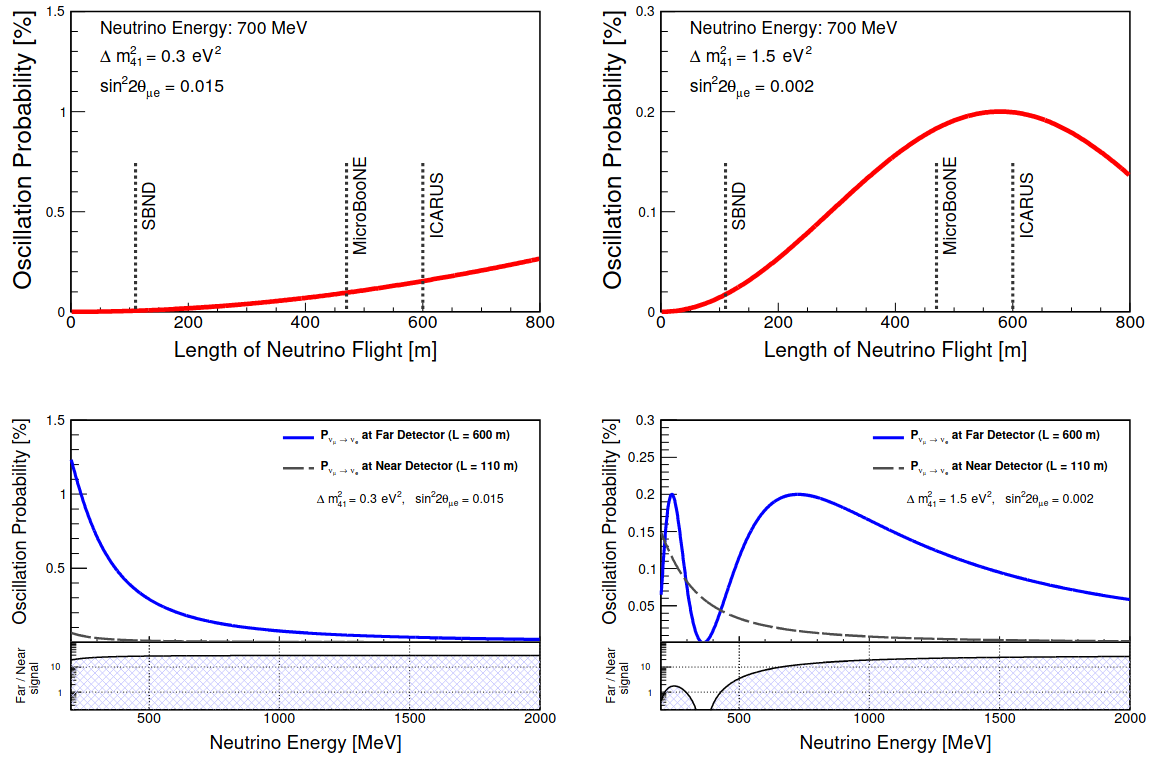
\includegraphics[width = \largefigwidth]{figures-chap3/osc_probability.png}
    \caption[SBN oscillation probability.]{The oscillation paramters used in the two left and right plots are $(sin^22\theta_{\mu e}, ~\Delta m^2_{41}) = (0.015, ~0.3~\text{eV}^2), (0.002, ~1.5~\text{eV}^2)$ respectively. Top: The oscillation probability as a function of the baseline for the \nue appearance channel. A neutrino energy of 700 MeV is used in both cases. Bottom: The oscillation probability is shown as a function of neutrino energy in both the near and far detector. Additionally, the ratio of the oscillation probabilities between the two detectors is also shown. \cite{SBN_paper}}
    \label{fig:osc_probability}
\end{figure}

\begin{figure}
    \centering
    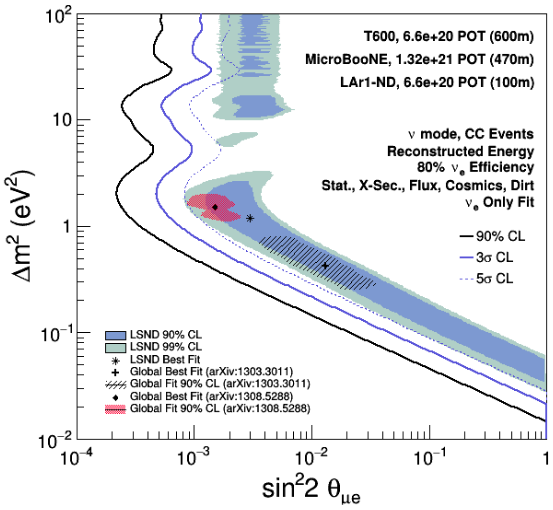
\includegraphics[width = \largefigwidth]{figures-chap3/SBN_proposal_sensitivity.png}
    \caption[\nue appearance\gls{sbn} proposal sensitivity.]{The expcted \nue appearance sensitivity from the \gls{sbn} program using inputs constructed at the time of the \gls{sbn} proposal. Limits from \gls{lsnd} and global best fit results are also shown \cite{SBN_Proposal}.}
    \label{fig:SBN_proposal_sensitivity}
\end{figure}

This main goal of the \gls{sbn} program revolves around sterile neutrino oscillation analyses, however the close proximity of the \gls{sbn} detectors and in particular \gls{sbnd} to the neutrino beam source will allow for a high statistics study of neutrino argon interactions. This will provide valuable information for future liquid argon based experiments such as \gls{dune}. \gls{sbnd} is expected to observe on the order of 2 million neutrino interactions a year which is sufficient to be able to minimise the associated uncertainty to a point such that systematic uncertainties become dominant. As the \gls{bnb} consists predominantly of \numu, most events will also be \numu based, however the \nue fraction of the \gls{bnb} is sufficient to expect 12,000 \nue events a year in \gls{sbnd} which is enough to perform both inclusive and exclusive analyses. There is also the opportunity to measure rare channels with a big increases in statistics or possibly even for the first time such as final states involving hyperons or $\nue \rightarrow \nue$ elastic scattering \cite{SBN_paper} \cite{light_dark_matter}.

The large event rate and the high resolution event reconstruction provided may allow the \gls{sbn} program to be sensitive to \gls{bsm} physics other than sterile neutrino oscillations \cite{SBN_paper}. The potential areas include, but are not limited to,
\begin{itemize}
    \item Light Dark Matter - Assuming a dark matter particle has an associated light mediator particle which interacts with quarks, the high intensity proton beam will produce a dark matter beam alongside neutrinos. The dark matter particles will propagate to the detectors alongside the neutrinos where they may scatter off the argon nuclei. Neutrinos will however represent a large background in such search \cite{SBN_paper}. 
    \item Large Extra Dimensions - The neutrino mass scale could be explained by the presence of additional dimensions. The right handed neutrinos would be able to propagate in the extra dimensions whilst the active neutrinos would be confined to the standard dimensions \cite{SBN_paper}. 
    \item Heavy Sterile Neutrinos - If heavy sterile neutrinos such as those present in the seesaw-mechanism discussed in \SectionRef{sec:seesaw_mechanism} are of an MeV mass scale, they may be produced in the \gls{bnb} vie meson decay. They would then propagate along the beam line and their decay products may observed in the detectors \cite{SBN_paper}\cite{MeV_scale_sterile_neutrino}.
    \item Dark Neutrinos - A beam neutrino interacts with an argon neucleus and scatters to a dark neutrino. The dark neutrino decays to a dark boson (and neutrino) and in turn the dark boson decays to an \positron \electron pair. This mechanism could provide an explanation to the \gls{miniboone} low energy excess \cite{SBN_paper}\cite{dark_neutrino}. 
\end{itemize}



            
            